\documentclass[10pt,a4paper]{article}
\usepackage[utf8]{inputenc}
\usepackage[T1]{fontenc}
\usepackage[margin=1in]{geometry}
\usepackage{graphicx}
\usepackage{booktabs} 
\usepackage{amsmath}   
\usepackage{siunitx}   
\usepackage[hidelinks]{hyperref}   
\usepackage{caption}   
\usepackage{float}    
\usepackage{microtype}
\usepackage{tikz}
\microtypesetup{expansion=false}

\title{\textbf{Structures}}
\author{Group 8}
\date{\today}

\begin{document}

\maketitle

\tableofcontents

\section{Introduction}
alalal


\newpage
\section{Deliverable 1: Geometry}
The roof geometry was reconstructed from the supplementary drawing using a one-to-one SketchUp model and then idealised for use in GSA. Figure~\ref{fig:geom_coordinates} shows the reconstructed nodal layout. Points labelled \textit{R} describe the roof profile, while points labelled \textit{S} describe the support system and the lower restraint points. The geometry is approximately symmetric about midspan, so the reconstructed coordinates were checked against the original drawing on both sides of the roof.

The overall geometric deviation of the reconstructed model is approximately 0.5\%. This difference is mainly due to manual scaling and point picking from the original drawing, but it is sufficiently small for the purposes of global structural modelling. The reconstructed geometry captures the changing roof curvature, the inclined support legs, and the position of the high nodes that anchor the main tie system.

\begin{figure}[H]
\centering
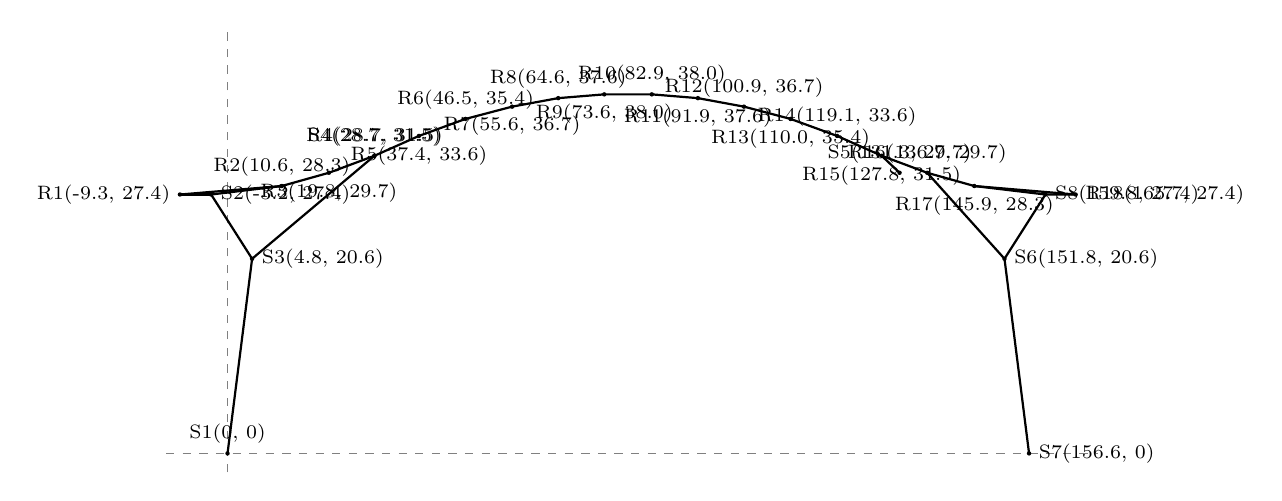
\begin{tikzpicture}[x=0.065cm,y=0.12cm,font=\scriptsize]
\draw[dashed,gray] (0,-2) -- (0,45);
\draw[dashed,gray] (-12,0) -- (170,0);

\coordinate (R1) at (-9.3,27.4);
\coordinate (R2) at (10.6,28.3);
\coordinate (R3) at (19.8,29.7);
\coordinate (R4) at (28.7,31.5);
\coordinate (R5) at (37.4,33.6);
\coordinate (R6) at (46.5,35.4);
\coordinate (R7) at (55.6,36.7);
\coordinate (R8) at (64.6,37.6);
\coordinate (R9) at (73.6,38.0);
\coordinate (R10) at (82.9,38.0);
\coordinate (R11) at (91.9,37.6);
\coordinate (R12) at (100.9,36.7);
\coordinate (R13) at (110.0,35.4);
\coordinate (R14) at (119.1,33.6);
\coordinate (R15) at (127.8,31.5);
\coordinate (R16) at (136.7,29.7);
\coordinate (R17) at (145.9,28.3);
\coordinate (R18) at (165.7,27.4);
\coordinate (S1) at (0,0);
\coordinate (S2) at (-3.2,27.4);
\coordinate (S3) at (4.8,20.6);
\coordinate (S4) at (28.7,31.5);
\coordinate (S5) at (131.3,29.7);
\coordinate (S6) at (151.8,20.6);
\coordinate (S7) at (156.6,0);
\coordinate (S8) at (159.8,27.4);

\draw[thick] (R1)--(R2)--(R3)--(R4)--(R5)--(R6)--(R7)--(R8)--(R9)--(R10)--(R11)--(R12)--(R13)--(R14)--(R15)--(R16)--(R17)--(R18);
\draw[thick] (S2)--(S3)--(S1);
\draw[thick] (S2)--(R2);
\draw[thick] (R1)--(S2);
\draw[thick] (S3)--(R4);
\draw[thick] (S4)--(R4);
\draw[thick] (S8)--(S6)--(S7);
\draw[thick] (R17)--(S8)--(R18);
\draw[thick] (S6)--(R16);
\draw[thick] (S5)--(R15);

\foreach \P in {R1,R2,R3,R4,R5,R6,R7,R8,R9,R10,R11,R12,R13,R14,R15,R16,R17,R18,S1,S2,S3,S4,S5,S6,S7,S8}
  \fill (\P) circle (0.8pt);

\node[anchor=east] at (R1) {R1(-9.3, 27.4)};
\node[anchor=south] at (R2) {R2(10.6, 28.3)};
\node[anchor=north] at (R3) {R3(19.8, 29.7)};
\node[anchor=south] at (R4) {R4(28.7, 31.5)};
\node[anchor=north] at (R5) {R5(37.4, 33.6)};
\node[anchor=south] at (R6) {R6(46.5, 35.4)};
\node[anchor=north] at (R7) {R7(55.6, 36.7)};
\node[anchor=south] at (R8) {R8(64.6, 37.6)};
\node[anchor=north] at (R9) {R9(73.6, 38.0)};
\node[anchor=south] at (R10) {R10(82.9, 38.0)};
\node[anchor=north] at (R11) {R11(91.9, 37.6)};
\node[anchor=south] at (R12) {R12(100.9, 36.7)};
\node[anchor=north] at (R13) {R13(110.0, 35.4)};
\node[anchor=south] at (R14) {R14(119.1, 33.6)};
\node[anchor=north] at (R15) {R15(127.8, 31.5)};
\node[anchor=south] at (R16) {R16(136.7, 29.7)};
\node[anchor=north] at (R17) {R17(145.9, 28.3)};
\node[anchor=west] at (R18) {R18(165.7, 27.4)};
\node[anchor=south] at (S1) {S1(0, 0)};
\node[anchor=west] at (S2) {S2(-3.2, 27.4)};
\node[anchor=west] at (S3) {S3(4.8, 20.6)};
\node[anchor=south] at (S4) {S4(28.7, 31.5)};
\node[anchor=south] at (S5) {S5(131.3, 29.7)};
\node[anchor=west] at (S6) {S6(151.8, 20.6)};
\node[anchor=west] at (S7) {S7(156.6, 0)};
\node[anchor=west] at (S8) {S8(159.8, 27.4)};
\end{tikzpicture}
\caption{Reconstructed geometry and nodal coordinates used to define the FE model}
\label{fig:geom_coordinates}
\end{figure}

Figure~\ref{fig:geom_members} shows the same geometry after it was converted into an FE idealisation. The curved top chord was divided into arch and tusk rafter segments, while the lower tie, straps, legs, wings and arms were represented as line members connected at the major nodes. This idealisation preserves the global load path of the real roof while remaining simple enough for efficient mesh refinement and sensitivity studies.

For the roof profile, each R-point corresponds to a measured section position along the curved rafter. In GSA, adjacent points were connected by straight beam elements, so the curved geometry is represented by a series of short linear segments. This is a standard approximation in frame modelling, and later mesh refinement was used to check that the adopted segmentation was sufficiently accurate.

\begin{figure}[H]
\centering
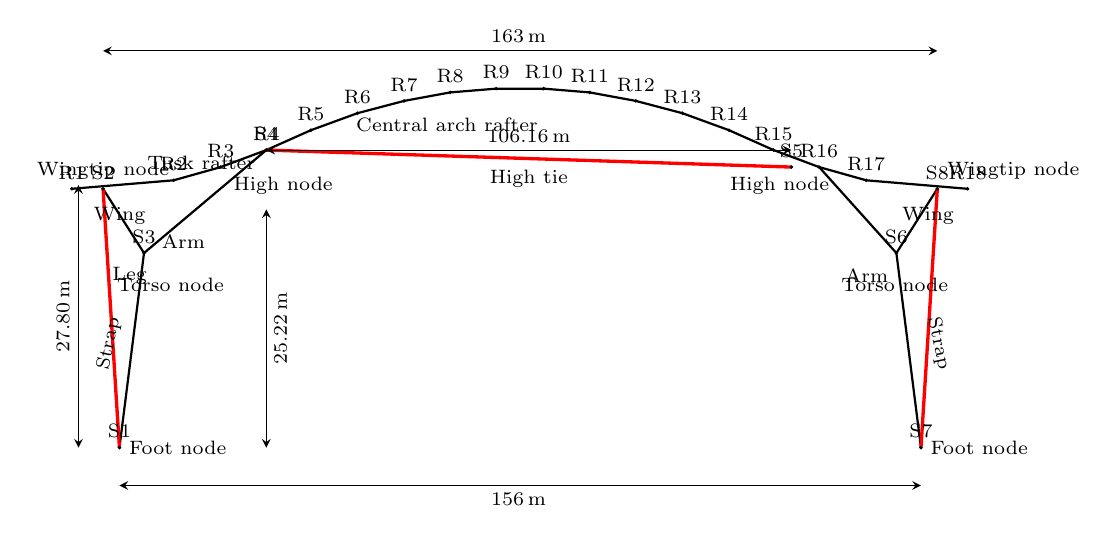
\begin{tikzpicture}[x=0.065cm,y=0.12cm,font=\scriptsize,>=stealth]
\coordinate (R1) at (-9.3,27.4);
\coordinate (R2) at (10.6,28.3);
\coordinate (R3) at (19.8,29.7);
\coordinate (R4) at (28.7,31.5);
\coordinate (R5) at (37.4,33.6);
\coordinate (R6) at (46.5,35.4);
\coordinate (R7) at (55.6,36.7);
\coordinate (R8) at (64.6,37.6);
\coordinate (R9) at (73.6,38.0);
\coordinate (R10) at (82.9,38.0);
\coordinate (R11) at (91.9,37.6);
\coordinate (R12) at (100.9,36.7);
\coordinate (R13) at (110.0,35.4);
\coordinate (R14) at (119.1,33.6);
\coordinate (R15) at (127.8,31.5);
\coordinate (R16) at (136.7,29.7);
\coordinate (R17) at (145.9,28.3);
\coordinate (R18) at (165.7,27.4);
\coordinate (S1) at (0,0);
\coordinate (S2) at (-3.2,27.4);
\coordinate (S3) at (4.8,20.6);
\coordinate (S4) at (28.7,31.5);
\coordinate (S5) at (131.3,29.7);
\coordinate (S6) at (151.8,20.6);
\coordinate (S7) at (156.6,0);
\coordinate (S8) at (159.8,27.4);

\draw[thick] (R1)--(R2)--(R3)--(R4)--(R5)--(R6)--(R7)--(R8)--(R9)--(R10)--(R11)--(R12)--(R13)--(R14)--(R15)--(R16)--(R17)--(R18);
\draw[thick] (S2)--(S3)--(S1);
\draw[thick] (S8)--(S6)--(S7);
\draw[thick] (S3)--(R4);
\draw[thick] (S6)--(R16);
\draw[red,very thick] (S2)--(S1);
\draw[red,very thick] (S8)--(S7);
\draw[red,very thick] (S4)--(S5);

\foreach \P/\L in {R1/R1,R2/R2,R3/R3,R4/R4,S4/S4,R5/R5,R6/R6,R7/R7,R8/R8,R9/R9,R10/R10,R11/R11,R12/R12,R13/R13,R14/R14,R15/R15,R16/R16,S5/S5,R17/R17,R18/R18,S1/S1,S2/S2,S3/S3,S6/S6,S7/S7,S8/S8}
{
  \fill (\P) circle (0.7pt);
  \node[anchor=south] at (\P) {\L};
}

\draw[<->] (-3.2,42) -- (159.8,42);
\node[fill=white,inner sep=1pt] at (78,43.5) {163\,m};
\draw[<->] (0,-4) -- (156.6,-4);
\node[fill=white,inner sep=1pt] at (78,-5.5) {156\,m};
\draw[<->] (28.7,31.5) -- (131.3,31.5);
\node[fill=white,inner sep=1pt] at (80,33.0) {106.16\,m};
\draw[<->] (-8,0) -- (-8,27.8);
\node[fill=white,inner sep=1pt,rotate=90] at (-11,13.9) {27.80\,m};
\draw[<->] (28.7,0) -- (28.7,25.22);
\node[fill=white,inner sep=1pt,rotate=90] at (31.5,12.6) {25.22\,m};
\node at (64,34.2) {Central arch rafter};
\node at (16,30.2) {Tusk rafter};
\node at (80,28.5) {High tie};
\node[rotate=78] at (-2,11) {Strap};
\node[rotate=-78] at (160,11) {Strap};
\node at (2,18.2) {Leg};
\node at (12.5,21.8) {Arm};
\node at (0,24.5) {Wing};
\node at (10,17.2) {Torso node};
\node at (32,27.7) {High node};
\node at (129,27.7) {High node};
\node at (146,18.2) {Arm};
\node at (158,24.5) {Wing};
\node at (151.5,17.2) {Torso node};
\node[anchor=west] at (S1) {Foot node};
\node[anchor=west] at (S7) {Foot node};
\node[anchor=south] at (S2) {Wingtip node};
\node[anchor=south west] at (S8) {Wingtip node};
\end{tikzpicture}
\caption{Idealised FE geometry showing the principal members and controlling dimensions}
\label{fig:geom_members}
\end{figure}

The final geometry model therefore provided both the coordinates needed for numerical analysis and a clear structural idealisation of the load-carrying system. These two figures were used as the basis for defining member connectivity, support positions, tie locations and the tributary frame width used in the later loading and sensitivity analysis.


\newpage
\section{Deliverable 2: Material, Section, and Loading Data }
The global FE model was defined using linear-elastic steel. In accordance with the coursework brief, all members were assigned an elastic modulus of \SI{200}{\giga\pascal}. A Poisson's ratio of 0.30 and density of \SI{7850}{\kilogram\per\metre\cubed} were adopted so that self-weight could be included automatically in GSA. S355 steel was used for the primary roof members, which is consistent with the Heathrow T5 project information. The high tie was modelled with an initial prestress of \SI{450}{\mega\pascal}.

Only vertical symmetric loading was considered. The characteristic permanent roof load was taken as the sum of the aluminium standing seam roof (\SI{0.10}{\kilo\pascal}), structural deck (\SI{0.15}{\kilo\pascal}), insulation/acoustic layers (\SI{0.40}{\kilo\pascal}) and services allowance (\SI{0.15}{\kilo\pascal}), giving $G_k = \SI{0.80}{\kilo\pascal}$. The characteristic imposed roof live load was taken as $Q_k = \SI{0.60}{\kilo\pascal}$. Therefore, the governing vertical ULS combination used in the model was
\[
1.35G_k + 1.5Q_k = 1.35(0.80) + 1.5(0.60) = \SI{1.98}{\kilo\pascal}.
\]
Using a tributary width of \SI{36}{\metre} for one transverse frame, this corresponds to an equivalent applied line load of \SI{71.28}{\kilo\newton\per\metre}, in addition to the self-weight of the primary members.

The strap members were modelled as rod elements. Therefore, only their axial stiffness was represented in the global model, using an equivalent steel area of $A = 2 \times 500 \times 40 = \SI{40000}{\milli\metre\squared}$. The spacing between the two plates was neglected in this idealisation because rod elements do not carry bending.

\begin{table}[H]
\centering
\caption{Section data adopted for the global model}
\label{tab:section_data}
\renewcommand{\arraystretch}{1.35}
\begin{tabular}{p{0.23\textwidth} p{0.32\textwidth} p{0.39\textwidth}}
\toprule
\textbf{Member} & \textbf{Section} & \textbf{Modelling note} \\
\midrule
Arch rafter & Welded box, \SI{800}{\milli\metre} wide, \SI{50}{\milli\metre} wall thickness & Depth varies from about \SI{1.8}{\metre} to \SI{3.8}{\metre} along the roof profile \\
Tusk rafter & Welded I-section, \SI{50}{\milli\metre} plate thickness & Overall depth varies from about \SI{0.9}{\metre} to \SI{3.8}{\metre} \\
Legs and arms & CHS \SI{914}{\milli\metre} $\times$ \SI{40}{\milli\metre} & Taken directly from the supplementary sketch \\
Wings & CHS \SI{711}{\milli\metre} $\times$ \SI{50}{\milli\metre} & Taken directly from the supplementary sketch \\
Internal/external ties & CHS \SI{457}{\milli\metre} $\times$ \SI{40}{\milli\metre} & Thickness not stated in the source, so \SI{40}{\milli\metre} was assumed \\
High tie & Twin locked-coil strands, $2 \times \SI{115}{\milli\metre}$ & Prestressed to \SI{450}{\mega\pascal} \\
Straps & Equivalent rod area \SI{40000}{\milli\metre\squared} & Based on two \SI{500}{\milli\metre} $\times$ \SI{40}{\milli\metre} plates; bending stiffness neglected \\
\bottomrule
\end{tabular}
\end{table}

The main assumptions were therefore a linear-elastic S355 steel model, uniform wall thickness where required by the brief, a \SI{36}{\metre} tributary width for each transverse frame, automatic inclusion of self-weight through the material density, and axial-only idealisation of the strap members.


\newpage
\section{Deliverable 3: Initial Model Validation}
\subsection{Assumptions}


\subsection{Model Validation}

\subsection{Model Adequacy}

\newpage
\section{Deliverable 4: Mesh Refinement Sensitivity Analysis}

\subsection{Introduction and Methodology}
In Finite Element Analysis (FEA), continuous curved geometries must be approximated using discrete straight beam elements. If the mesh is too coarse, the structural stiffness and internal bending moments of curved members are inaccurately represented. A sensitivity study was conducted to determine the optimum mesh density that provides mathematical convergence without introducing unnecessary computational expense. 

The study selectively targeted the continuous curved roof profile, specifically the Arch and Tusk Rafters (including the cantilevered eaves). These members carry heavy distributed loads ($72.74 \text{ kN/m}$) and are subjected to complex bending forces. Conversely, the straight high ties and the vertical abutment columns (legs and arms) were excluded from the refinement process; as primarily axially loaded members, their behaviour is perfectly captured by single elements between major nodes regardless of mesh density.

\subsection{Mesh Definitions}
Three levels of mesh refinement were analysed under the critical ULS vertical load combination ($1.35G_k + 1.5Q_k$) and the $450 \text{ MPa}$ high tie prestress. The base geometry was defined by the 16 coordinate nodes provided in the project data.

The baseline geometry of Mesh 1 (coarse) consisting of 1 element per original coordinate segment across the roof profile. (Average arch element length $\approx 2.5 \text{ m}$). For Mesh 2 (medium), all elements along the continuous roof profile were split into two equal segments. (Average arch element length $\approx 1.25 \text{ m}$). For Mesh 3 (fine), all elements along the continuous roof profile were split again into two equal segments, resulting in four elements per original coordinate segment. (Average arch element length $\approx 0.6 \text{ m}$).

\subsection{Comparison of Key Response Quantities}
To evaluate convergence, three critical structural responses were monitored across the three models, maximum vertical deflection ($\delta_z$), which was measured at the crown (apex) of the arch rafter, maximum bending moment ($M_y$) measured within the arch rafter, and maximum axial tension ($F_x$), which is measured in the main twin high tie.

\begin{table}[h]
\centering
\caption{Mesh Sensitivity Results under ULS Loading}
\vspace{0.2cm}
\label{tab:mesh_sensitivity}
\renewcommand{\arraystretch}{1.5}
\resizebox{\textwidth}{!}{
\begin{tabular}{|l|c|c|c|c|}
\hline
\textbf{Parameter} & \textbf{Mesh 1 (Coarse)} & \textbf{Mesh 2 (Medium)} & \textbf{Mesh 3 (Fine)} & \textbf{\% Change (Med to Fine)} \\ \hline
\textbf{Max Crown Deflection (mm)} & [Output] & [Output] & [Output] & [\%] \\ \hline
\textbf{Max Arch Bending Moment (kNm)} & [Output] & [Output] & [Output] & [\%] \\ \hline
\textbf{High Tie Axial Force (kN)} & [Output] & [Output] & [Output] & [\%] \\ \hline
\end{tabular}
}
\end{table}

\subsection{Conclusion and Adopted Mesh Density}
As demonstrated in Table \ref{tab:mesh_sensitivity}, transitioning from the coarse mesh to the medium mesh resulted in noticeable changes to the internal forces and deflections. This indicates that the coarse mesh artificially bridges the true curvature of the arch, creating an overly stiff model that inaccurately distributes bending moments.

However, further refinement from the medium mesh to the fine mesh yielded a negligible variance of [ \% ] in the key response quantities. This demonstrates that the FE results have converged and the global behaviour of the structure is no longer highly sensitive to element size.

Therefore, Mesh 2 (medium mesh) provides sufficient geometric accuracy for the purpose of global structural modelling. It captures the true bending behaviour of the sweeping arch rafters without introducing the unnecessary mathematical complexity of Mesh 3. Mesh 2 has been adopted for all subsequent global analyses in this report.

\newpage
\section{Deliverable 6: Boundary Conditions for More Detailed Analysis}

For a more detailed FE study, the rafter splice between the tusk rafter and arch rafter should be extracted from the global frame model and analysed as a local submodel. The purpose of the local model would be to resolve the stress distribution in the splice plates, bolts or welds, and the adjacent box and I-section walls, which cannot be captured accurately by the beam idealisation used in the global model.

The local model should include a short length of member on each side of the splice so that the boundary conditions are applied away from the connection itself. This reduces artificial stress concentrations caused by restraining the model too close to the detail. A practical choice would be to include approximately one section depth of the arch rafter and one section depth of the tusk rafter beyond the splice on either side.

\begin{figure}[H]
\centering
\fbox{
\begin{minipage}{0.9\textwidth}
\centering
\small
\begin{tabular}{c c c}
Arch rafter cut face & Splice region & Tusk rafter cut face \\
\rule{0.22\textwidth}{0.4pt} & \fbox{\parbox{0.20\textwidth}{\centering splice plates\\ bolts / welds}} & \rule{0.22\textwidth}{0.4pt} \\
$u_x,u_y,u_z,r_x,r_y,r_z$ & local solid/shell model & $u_x,u_y,u_z,r_x,r_y,r_z$ \\
from global model &  & from global model \\
\end{tabular}
\end{minipage}
}
\caption{Recommended boundary conditions for the local splice model}
\label{fig:splice_bc}
\end{figure}

The preferred boundary condition is to impose the displacement and rotation components extracted from the global beam model at the two cut faces of the local model. In practice, each cut face can be coupled to a reference node so that the sectional deformation remains compatible with the global model. The six kinematic quantities imposed at each end are the three translations ($u_x$, $u_y$, $u_z$) and the three rotations ($r_x$, $r_y$, $r_z$). This approach is preferable to simply fixing one end, because it reproduces the actual deformation state of the connection and avoids introducing artificial restraint moments.

The corresponding section forces should also be checked against the global model outputs. The main actions expected at the splice are axial force $N$, vertical shear $V$, bending moment $M$, and a smaller torsional component due to the curved roof geometry and eccentricity of the connection detail. If the software or modelling approach makes direct displacement transfer difficult, an acceptable alternative is to apply the equivalent set of sectional resultants at the two cut faces, provided that overall equilibrium is maintained.

To prevent rigid body motion in the local model, one reference node may be lightly stabilised after the global displacements have been assigned. This stabilisation should only remove numerical singularities and must not alter the transferred load path. Contact, bolt preload, or weld representation can then be added depending on the intended level of detail. For the purposes of this coursework, the key requirement is that the splice boundaries are driven by the global model response rather than by arbitrary fixed supports.
\end{document}
